\documentclass[sumario=abnt-6027-2012]{ifes8}

\usepackage[utf8]{inputenc}
\usepackage{graphicx}
\usepackage{float}
\usepackage{array}
\usepackage{booktabs}
\usepackage{url}
\usepackage{amssymb}
\usepackage{amsmath}
\usepackage{tikz}
\usetikzlibrary{automata,positioning,arrows}

\tikzset{
  >=stealth',
  initial text={},
  every state/.style={draw, circle, minimum size=1.0cm, font=\small},
}

% -----------------------------------------------------------------
\titulo{Laboratório 01: Linguagens Regulares}
\autor{Flávio Miozzi Batista}
\local{Serra}
\data{2026}
\orientador{Prof. Jefferson Oliveira Andrade}
\instituicao{Instituto Federal do Espírito Santo}
\curso{Mestrado Profissional em Computação Aplicada}
\preambulo{Relatório de atividade de laboratório apresentado ao
  Mestrado Profissional em Computação Aplicada do Instituto Federal do
  Espírito Santo como parte das atividades da disciplina Teoria da
  Computação, semestre 2026/1, sob orientação do
  Prof.\ Jefferson Oliveira Andrade.}

% -----------------------------------------------------------------
\newcommand{\rx}[1]{\texttt{#1}}
\newcommand{\celula}[1]{\textbf{#1}}
\newcommand{\heart}{\ensuremath{\heartsuit}}
\newcommand{\eps}{\varepsilon}

% -----------------------------------------------------------------
\begin{document}

\imprimircapa

\begin{folhaderosto}
\end{folhaderosto}

\pdfbookmark[0]{\contentsname}{toc}
\tableofcontents*
\cleardoublepage

\textual

% =================================================================
\chapter{Introdução}
% =================================================================

Este relatório documenta as três partes do Laboratório~01 da disciplina
Teoria da Computação do PPCOMPI/IFES.

A \textbf{Parte~1} trata da conversão de Autômatos Finitos Não-Determinísticos
com transições~$\varepsilon$ (NFA$\varepsilon$) para Autômatos Finitos Determinísticos
Mínimos (DFA), por meio de três etapas: remoção de transições~$\varepsilon$,
construção de subconjuntos e minimização pelo algoritmo de Hopcroft.
A implementação encontra-se em \texttt{Main.hs}.

A \textbf{Parte~2} aborda a construção de Thompson, que converte uma expressão
regular em um NFA$\varepsilon$, o qual é então convertido para DFA mínimo pelo mesmo
pipeline da Parte~1. A implementação encontra-se em \texttt{Regex.hs}.

A \textbf{Parte~3} apresenta soluções para a plataforma \textit{Regex
Crossword}, que exercita a leitura e escrita de expressões regulares.

% =================================================================
\chapter{Parte 1 --- Conversão de Autômatos Finitos}
% =================================================================

\section{Visão Geral do Algoritmo}

A conversão NFA$\varepsilon$ $\to$ DFA mínimo implementada em \texttt{Main.hs} realiza
três etapas sequenciais:

\begin{enumerate}
  \item \textbf{Remoção de transições $\varepsilon$:} para cada estado $q$,
    computa-se o $\varepsilon$-fecho $\overline{\varepsilon}(q)$ — o conjunto
    de estados alcançáveis a partir de $q$ por zero ou mais transições
    $\varepsilon$. As transições do novo NFA são redefinidas incorporando
    esses fechos.
  \item \textbf{Construção de subconjuntos (\textit{subset construction}):}
    os estados do DFA são subconjuntos de estados do NFA. O DFA inicial
    corresponde ao $\varepsilon$-fecho do estado inicial do NFA, e as
    transições são computadas iterativamente até que nenhum novo subconjunto
    seja gerado.
  \item \textbf{Minimização por Hopcroft:} o DFA resultante é minimizado
    usando o algoritmo de Hopcroft, que particiona os estados em classes de
    equivalência com base na distinguibilidade por strings de entrada.
\end{enumerate}

\section{Exemplo 1 --- \texttt{nfae\_simple} ($L = 0^*1$)}

O autômato \texttt{nfae\_simple} possui 3~estados sobre o alfabeto
$\Sigma = \{0, 1\}$ e reconhece $L = 0^*1$ (zero ou mais $0$s seguidos de
exatamente um $1$). A transição $\varepsilon$ de $q_0$ para $q_1$ permite
que o autômato ``pule'' diretamente para o estado que aguarda o símbolo~$1$.

\begin{figure}[H]
  \centering
  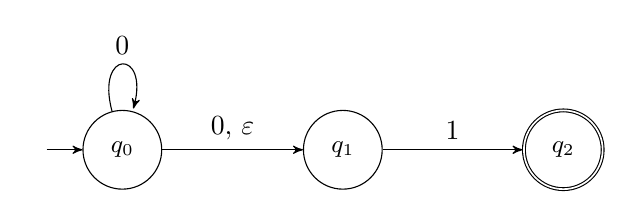
\begin{tikzpicture}[->, node distance=2.8cm, auto]
    \node[state, initial]    (q0) {$q_0$};
    \node[state]             (q1) [right of=q0] {$q_1$};
    \node[state, accepting]  (q2) [right of=q1] {$q_2$};
    \path
      (q0) edge [loop above] node {$0$} ()
      (q0) edge node {$0,\,\eps$} (q1)
      (q1) edge node {$1$} (q2);
  \end{tikzpicture}
  \caption{NFA$\varepsilon$ \texttt{nfae\_simple}: estado inicial $q_0$, estado final $q_2$.}
  \label{fig:nfae-simple-nfae}
\end{figure}

Após a remoção das transições~$\varepsilon$, o NFA equivalente consolida o
comportamento de $q_0$ absorvendo as transições de $q_1$:

\begin{figure}[H]
  \centering
  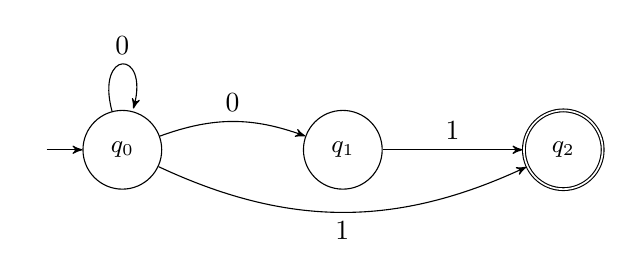
\begin{tikzpicture}[->, node distance=2.8cm, auto]
    \node[state, initial]    (q0) {$q_0$};
    \node[state]             (q1) [right of=q0] {$q_1$};
    \node[state, accepting]  (q2) [right of=q1] {$q_2$};
    \path
      (q0) edge [loop above] node {$0$} ()
      (q0) edge [bend left=20]  node [above] {$0$} (q1)
      (q0) edge [bend right=25] node [below] {$1$} (q2)
      (q1) edge node {$1$} (q2);
  \end{tikzpicture}
  \caption{NFA intermediário (sem transições~$\varepsilon$).}
  \label{fig:nfae-simple-nfa}
\end{figure}

O DFA mínimo resultante possui apenas 2~estados: o estado
$\{q_0\}$ (inicial, não-final) e $\{q_2\}$ (final). O estado morto
implícito, para entradas após $\{q_2\}$, é eliminado pela minimização.

\begin{figure}[H]
  \centering
  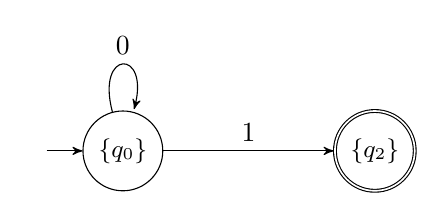
\begin{tikzpicture}[->, node distance=3.2cm, auto]
    \node[state, initial]    (A) {$\{q_0\}$};
    \node[state, accepting]  (B) [right of=A] {$\{q_2\}$};
    \path
      (A) edge [loop above] node {$0$} ()
      (A) edge node {$1$} (B);
  \end{tikzpicture}
  \caption{DFA mínimo: $L = 0^*1$.}
  \label{fig:nfae-simple-dfa}
\end{figure}

% -----------------------------------------------------------------
\section{Exemplo 2 --- \texttt{nfae\_02} ($L = \{a,b\}$)}

O autômato \texttt{nfae\_02} possui 5~estados, usa transições~$\varepsilon$
para modelar a escolha não-determinística entre $a$ e $b$, e reconhece
$L = \{a, b\}$ (exatamente uma letra).

\begin{figure}[H]
  \centering
  \begin{tikzpicture}[->, node distance=1.9cm, auto]
    \node[state, initial] (q0) {$q_0$};
    \node[state] (q1) [above right=1.2cm and 2cm of q0] {$q_1$};
    \node[state] (q2) [below right=1.2cm and 2cm of q0] {$q_2$};
    \node[state] (q3) [below right=1.2cm and 2cm of q1] {$q_3$};
    \node[state, accepting] (q4) [right=2.2cm of q3] {$q_4$};
    \path
      (q0) edge node [above left]  {$\eps$} (q1)
      (q0) edge node [below left]  {$\eps$} (q2)
      (q1) edge node [above right] {$a$}    (q3)
      (q2) edge node [below right] {$b$}    (q3)
      (q3) edge node               {$\eps$} (q4);
  \end{tikzpicture}
  \caption{NFA$\varepsilon$ \texttt{nfae\_02}: $L = \{a, b\}$.}
  \label{fig:nfae02-nfae}
\end{figure}

O DFA mínimo colapsa todos os estados intermediários em dois estados:

\begin{figure}[H]
  \centering
  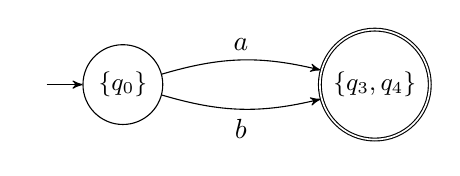
\begin{tikzpicture}[->, node distance=3.2cm, auto]
    \node[state, initial]    (A) {$\{q_0\}$};
    \node[state, accepting]  (B) [right of=A] {$\{q_3,q_4\}$};
    \path
      (A) edge [bend left=15]  node [above] {$a$} (B)
      (A) edge [bend right=15] node [below] {$b$} (B);
  \end{tikzpicture}
  \caption{DFA mínimo: $L = \{a, b\}$.}
  \label{fig:nfae02-dfa}
\end{figure}

% -----------------------------------------------------------------
\section{Exemplo 3 --- \texttt{nfae\_04} ($L = \{ab\}$)}

O autômato \texttt{nfae\_04} possui 4~estados e reconhece $L = \{ab\}$
(somente a cadeia ``ab''). A transição~$\varepsilon$ entre $q_1$ e $q_2$
serve como conector entre os dois estágios de leitura.

\begin{figure}[H]
  \centering
  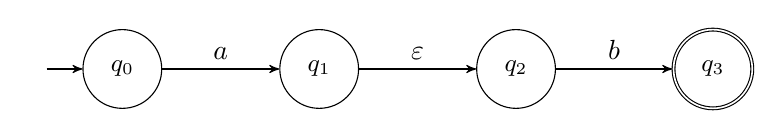
\begin{tikzpicture}[->, node distance=2.5cm, auto]
    \node[state, initial]    (q0) {$q_0$};
    \node[state]             (q1) [right of=q0] {$q_1$};
    \node[state]             (q2) [right of=q1] {$q_2$};
    \node[state, accepting]  (q3) [right of=q2] {$q_3$};
    \path
      (q0) edge node {$a$}    (q1)
      (q1) edge node {$\eps$} (q2)
      (q2) edge node {$b$}    (q3);
  \end{tikzpicture}
  \caption{NFA$\varepsilon$ \texttt{nfae\_04}: $L = \{ab\}$.}
  \label{fig:nfae04-nfae}
\end{figure}

Após a construção de subconjuntos, o estado $\{q_1, q_2\}$ surge porque
$q_2$ pertence ao $\varepsilon$-fecho de $q_1$.

\begin{figure}[H]
  \centering
  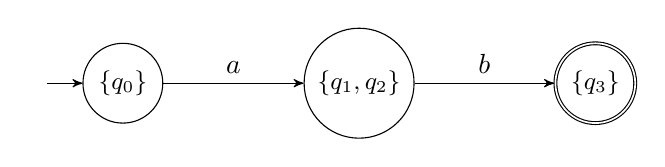
\begin{tikzpicture}[->, node distance=3.0cm, auto]
    \node[state, initial]    (A) {$\{q_0\}$};
    \node[state]             (B) [right of=A] {$\{q_1,q_2\}$};
    \node[state, accepting]  (C) [right of=B] {$\{q_3\}$};
    \path
      (A) edge node {$a$} (B)
      (B) edge node {$b$} (C);
  \end{tikzpicture}
  \caption{DFA mínimo: $L = \{ab\}$.}
  \label{fig:nfae04-dfa}
\end{figure}

% -----------------------------------------------------------------
\section{Exemplo 4 --- \texttt{nfae\_06} ($L = (a|b)^*$)}

O autômato \texttt{nfae\_06} é a construção de Thompson para
$(a|b)^*$, com 8~estados. O estado inicial $q_0$ possui transições~$\varepsilon$
diretas para $q_1$ (ramo interno do Kleene) e $q_7$ (estado final, para aceitar
a cadeia vazia). O ciclo $q_6 \to q_1$ implementa a repetição.

\begin{figure}[H]
  \centering
  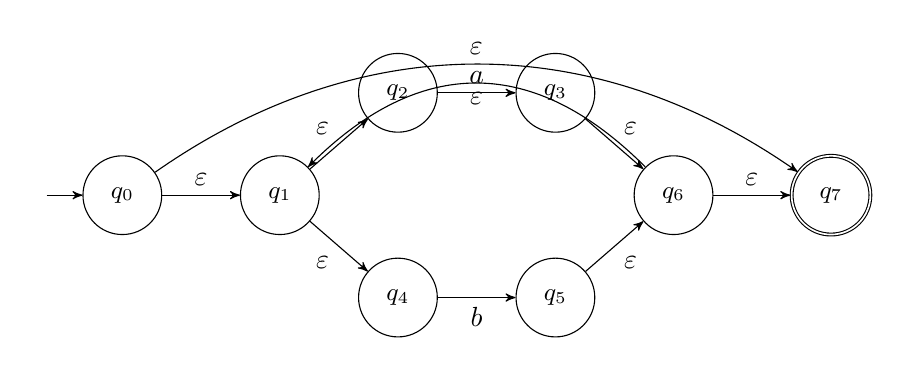
\begin{tikzpicture}[->, auto]
    \node[state, initial] (q0) at (0,0)    {$q_0$};
    \node[state]          (q1) at (2,0)    {$q_1$};
    \node[state]          (q2) at (3.5,1.3){$q_2$};
    \node[state]          (q3) at (5.5,1.3){$q_3$};
    \node[state]          (q4) at (3.5,-1.3){$q_4$};
    \node[state]          (q5) at (5.5,-1.3){$q_5$};
    \node[state]          (q6) at (7,0)    {$q_6$};
    \node[state, accepting](q7) at (9,0)   {$q_7$};
    \path
      (q0) edge node [above]       {$\eps$} (q1)
      (q0) edge [bend left=35]
                node [above]       {$\eps$} (q7)
      (q1) edge node [above left]  {$\eps$} (q2)
      (q1) edge node [below left]  {$\eps$} (q4)
      (q2) edge node [above]       {$a$}    (q3)
      (q3) edge node [above right] {$\eps$} (q6)
      (q4) edge node [below]       {$b$}    (q5)
      (q5) edge node [below right] {$\eps$} (q6)
      (q6) edge node [above]       {$\eps$} (q7)
      (q6) edge [bend right=45, looseness=1.2]
                node [below]       {$\eps$} (q1);
  \end{tikzpicture}
  \caption{NFA$\varepsilon$ \texttt{nfae\_06} (construção de Thompson para $(a|b)^*$).}
  \label{fig:nfae06-nfae}
\end{figure}

Como $(a|b)^*$ aceita qualquer cadeia sobre $\{a,b\}$, o DFA mínimo
colapsa para um único estado, inicial e final, com auto-laços em $a$ e $b$:

\begin{figure}[H]
  \centering
  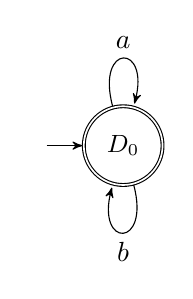
\begin{tikzpicture}[->, node distance=2.5cm, auto]
    \node[state, initial, accepting] (D) {$D_0$};
    \path
      (D) edge [loop above] node {$a$} ()
      (D) edge [loop below] node {$b$} ();
  \end{tikzpicture}
  \caption{DFA mínimo: $L = (a|b)^*$ (estado único, inicial e final).}
  \label{fig:nfae06-dfa}
\end{figure}

% -----------------------------------------------------------------
\section{Exemplo 5 --- \texttt{nfae\_complex}}

O autômato \texttt{nfae\_complex} possui 13~estados sobre
$\Sigma = \{a,b,c\}$ e reconhece cadeias que: (i)~começam com $ab$ ou $cb$;
(ii)~contêm ao menos um $c$ intermediário; e (iii)~terminam com $ba$ ou $cc$.

A Figura~\ref{fig:nfae-complex-nfae} apresenta o diagrama do NFA$\varepsilon$, onde
o par $(q_0 \to q_1 \to q_2, \; q_0 \to q_3 \to q_4) \to q_5$ codifica
os prefixos alternativos, $q_6$ e $q_7$ modelam o meio da cadeia, e os
sufixos $ba$ e $cc$ são capturados por $(q_8, q_9)$ e $(q_{10}, q_{11})$,
respectivamente, convergindo para $q_{12}$.

\begin{figure}[H]
  \centering
  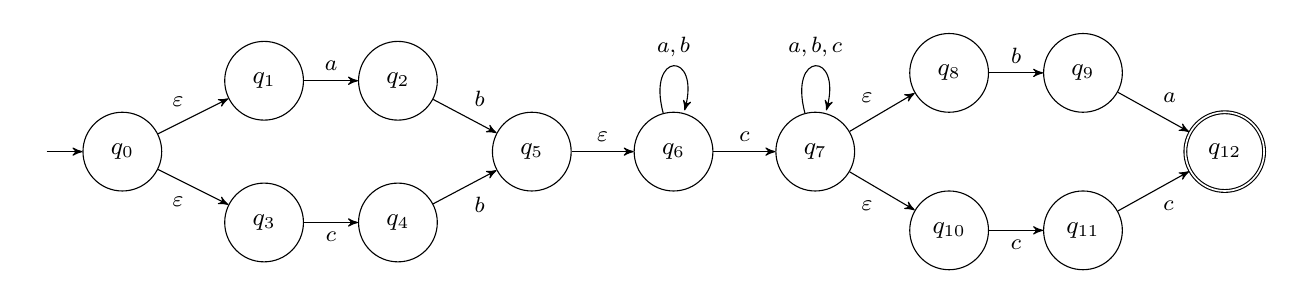
\begin{tikzpicture}[->, auto, font=\footnotesize]
    % Prefixo
    \node[state, initial] (q0) at (0,0)     {$q_0$};
    \node[state]          (q1) at (1.8,0.9) {$q_1$};
    \node[state]          (q3) at (1.8,-0.9){$q_3$};
    \node[state]          (q2) at (3.5,0.9) {$q_2$};
    \node[state]          (q4) at (3.5,-0.9){$q_4$};
    \node[state]          (q5) at (5.2,0)   {$q_5$};
    % Meio
    \node[state]          (q6) at (7,0)     {$q_6$};
    \node[state]          (q7) at (8.8,0)   {$q_7$};
    % Sufixos
    \node[state]          (q8)  at (10.5,1.0)  {$q_8$};
    \node[state]          (q9)  at (12.2,1.0)  {$q_9$};
    \node[state]          (q10) at (10.5,-1.0) {$q_{10}$};
    \node[state]          (q11) at (12.2,-1.0) {$q_{11}$};
    \node[state, accepting](q12) at (14,0)    {$q_{12}$};
    \path
      (q0) edge node [above left]  {$\eps$} (q1)
      (q0) edge node [below left]  {$\eps$} (q3)
      (q1) edge node [above]       {$a$}    (q2)
      (q3) edge node [below]       {$c$}    (q4)
      (q2) edge node [above right] {$b$}    (q5)
      (q4) edge node [below right] {$b$}    (q5)
      (q5) edge node               {$\eps$} (q6)
      (q6) edge [loop above] node  {$a,b$}  ()
      (q6) edge node [above]       {$c$}    (q7)
      (q7) edge [loop above] node  {$a,b,c$}()
      (q7) edge node [above left]  {$\eps$} (q8)
      (q7) edge node [below left]  {$\eps$} (q10)
      (q8) edge node [above]       {$b$}    (q9)
      (q9) edge node [above right] {$a$}    (q12)
      (q10) edge node [below]      {$c$}    (q11)
      (q11) edge node [below right]{$c$}    (q12);
  \end{tikzpicture}
  \caption{NFA$\varepsilon$ \texttt{nfae\_complex} (13~estados, $\Sigma = \{a,b,c\}$).}
  \label{fig:nfae-complex-nfae}
\end{figure}

A construção de subconjuntos seguida de minimização produz um DFA com
8~estados. A Tabela~\ref{tab:complex-estados} define a correspondência entre
os estados renomeados ($D_0$--$D_7$) e os subconjuntos de estados do NFA.

\begin{table}[H]
  \centering
  \caption{Correspondência de estados — DFA de \texttt{nfae\_complex}.}
  \label{tab:complex-estados}
  \begin{tabular}{clc}
    \toprule
    \textbf{Estado DFA} & \textbf{Subconjunto NFA} & \textbf{Final?} \\
    \midrule
    $D_0$ & $\{q_0\}$                              & Não \\
    $D_1$ & $\{q_2\}$                              & Não \\
    $D_2$ & $\{q_6\}$                              & Não \\
    $D_3$ & $\{q_6,q_7,q_8,q_{10}\}$              & Não \\
    $D_4$ & $\{q_6,q_7,q_8,q_{10},q_{11}\}$       & Não \\
    $D_5$ & $\{q_6,q_7,q_8,q_9,q_{10}\}$          & Não \\
    $D_6$ & $\{q_6,q_7,q_8,q_{10},q_{11},q_{12}\}$& \textbf{Sim} \\
    $D_7$ & $\{q_6,q_7,q_8,q_{10},q_{12}\}$       & \textbf{Sim} \\
    \bottomrule
  \end{tabular}
\end{table}

\begin{table}[H]
  \centering
  \caption{Tabela de transições do DFA mínimo de \texttt{nfae\_complex}.
           O símbolo ``$\emptyset$'' indica transição para o estado morto
           (eliminado pela minimização).}
  \label{tab:complex-trans}
  \renewcommand{\arraystretch}{1.2}
  \begin{tabular}{ccccc}
    \toprule
    \textbf{Estado} & \textbf{Final?} & $a$ & $b$ & $c$ \\
    \midrule
    $\to D_0$ &     & $D_1$       & $\emptyset$ & $D_1$ \\
    $D_1$     &     & $\emptyset$ & $D_2$       & $\emptyset$ \\
    $D_2$     &     & $D_2$       & $D_2$       & $D_3$ \\
    $D_3$     &     & $D_3$       & $D_5$       & $D_4$ \\
    $D_4$     &     & $D_3$       & $D_5$       & $D_6$ \\
    $D_5$     &     & $D_7$       & $D_5$       & $D_4$ \\
    $D_6$     & $*$ & $D_3$       & $D_5$       & $D_6$ \\
    $D_7$     & $*$ & $D_3$       & $D_5$       & $D_4$ \\
    \bottomrule
  \end{tabular}
\end{table}

% =================================================================
\chapter{Parte 2 --- Expressões Regulares}
% =================================================================

\section{Visão Geral --- Construção de Thompson}

O módulo \texttt{Regex.hs} implementa a conversão de uma expressão regular
para DFA mínimo em quatro estágios:

\begin{enumerate}
  \item \textbf{Análise sintática (\textit{parsing}):} a expressão regular é
    lida como string e convertida para uma árvore sintática abstrata (AST)
    usando combinadores de \textit{parsing} em Haskell.
  \item \textbf{Construção de Thompson:} a AST é percorrida
    recursivamente, gerando um NFA$\varepsilon$ por indução estrutural — concatenação,
    alternância ($|$), Kleene ($*$/$+$) e opção ($?$) possuem construções
    padrão.
  \item \textbf{Eliminação de $\varepsilon$ e construção de subconjuntos:}
    o NFA$\varepsilon$ gerado é passado ao mesmo pipeline de \texttt{Main.hs}.
  \item \textbf{Minimização de Hopcroft:} o DFA resultante é minimizado.
\end{enumerate}

Para cada expressão regular a seguir, apresenta-se a expressão, a linguagem
reconhecida e o DFA mínimo obtido, com renomeação dos estados por clareza.

% -----------------------------------------------------------------
\section{Expressão 1 --- \rx{ab*}}

A expressão \rx{ab*} denota $L = \{ab^n \mid n \geq 0\} = a \cdot b^*$:
uma cadeia começa com exatamente um $a$, seguido de zero ou mais $b$s.
O DFA mínimo possui 2~estados.

\begin{figure}[H]
  \centering
  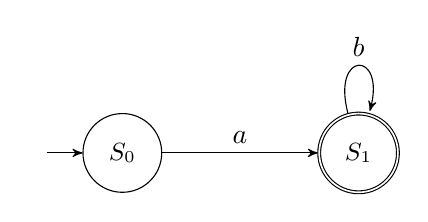
\begin{tikzpicture}[->, node distance=3.0cm, auto]
    \node[state, initial]   (S0) {$S_0$};
    \node[state, accepting] (S1) [right of=S0] {$S_1$};
    \path
      (S0) edge node {$a$} (S1)
      (S1) edge [loop above] node {$b$} ();
  \end{tikzpicture}
  \caption{DFA mínimo para \rx{ab*}: $S_0 = \{q_0\}$,
           $S_1 = \{q_3,q_4,q_5\}$.}
  \label{fig:dfa-regex1}
\end{figure}

% -----------------------------------------------------------------
\section{Expressão 2 --- \rx{a*b+}}

A expressão \rx{a*b+} denota $L = a^* \cdot b^+$: zero ou mais $a$s
seguidos de ao menos um $b$. O DFA mínimo possui 2~estados.

\begin{figure}[H]
  \centering
  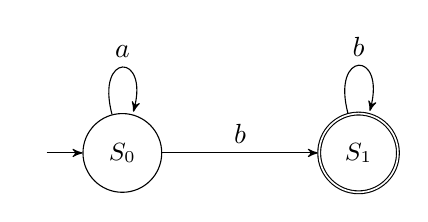
\begin{tikzpicture}[->, node distance=3.0cm, auto]
    \node[state, initial]   (S0) {$S_0$};
    \node[state, accepting] (S1) [right of=S0] {$S_1$};
    \path
      (S0) edge [loop above] node {$a$} ()
      (S0) edge node {$b$} (S1)
      (S1) edge [loop above] node {$b$} ();
  \end{tikzpicture}
  \caption{DFA mínimo para \rx{a*b+}: $S_0 = \{q_0\}$,
           $S_1 = \{q_7,q_8,q_9\}$.}
  \label{fig:dfa-regex2}
\end{figure}

% -----------------------------------------------------------------
\section{Expressão 3 --- \rx{(a|b)*abb}}

A expressão \rx{(a|b)*abb} denota $L = (a|b)^* \cdot abb$: todas as cadeias
sobre $\{a,b\}$ que terminam com o sufixo $abb$. Este é o exemplo clássico
de 4~estados que ilustra o DFA da construção de subconjuntos.

\begin{figure}[H]
  \centering
  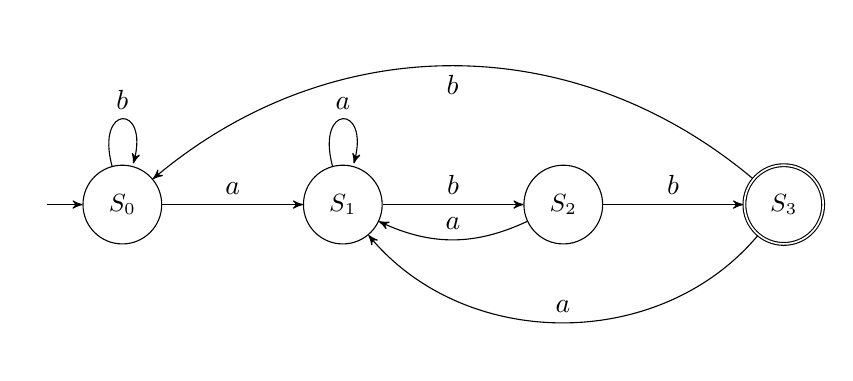
\begin{tikzpicture}[->, node distance=2.8cm, auto]
    \node[state, initial]   (S0) {$S_0$};
    \node[state]            (S1) [right of=S0] {$S_1$};
    \node[state]            (S2) [right of=S1] {$S_2$};
    \node[state, accepting] (S3) [right of=S2] {$S_3$};
    \path
      (S0) edge [loop above] node {$b$} ()
      (S0) edge node {$a$} (S1)
      (S1) edge [loop above] node {$a$} ()
      (S1) edge node {$b$} (S2)
      (S2) edge [bend left=25] node [above] {$a$} (S1)
      (S2) edge node {$b$} (S3)
      (S3) edge [bend right=40] node [below] {$b$} (S0)
      (S3) edge [bend left=50] node [above] {$a$} (S1);
  \end{tikzpicture}
  \caption{DFA mínimo para \rx{(a|b)*abb}.
    $S_0=\{q_0\}$; $S_1=\{q_1,q_2,q_3,q_4,q_5,q_6,q_8,q_9,q_{10}\}$;
    $S_2=\{q_1,q_2,q_3,q_4,q_6,q_7,q_8,q_{11},q_{12}\}$;
    $S_3=\{q_1,q_2,q_3,q_4,q_6,q_7,q_8,q_{13}\}^*$.}
  \label{fig:dfa-regex3}
\end{figure}

% -----------------------------------------------------------------
\section{Expressão 4 --- \rx{a?}}

A expressão \rx{a?} denota $L = \{\varepsilon, a\}$: a cadeia vazia ou
exatamente um $a$. Como o alfabeto de entrada é $\{a\}$, o DFA mínimo
possui 2~estados, ambos finais (a cadeia vazia é aceita pelo estado
inicial).

\begin{figure}[H]
  \centering
  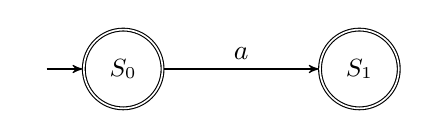
\begin{tikzpicture}[->, node distance=3.0cm, auto]
    \node[state, initial, accepting] (S0) {$S_0$};
    \node[state, accepting]          (S1) [right of=S0] {$S_1$};
    \path
      (S0) edge node {$a$} (S1);
  \end{tikzpicture}
  \caption{DFA mínimo para \rx{a?}: $S_0 = \{q_0\}$, $S_1 = \{q_1,q_3\}$.
           Ambos os estados são finais; $S_1$ não possui transições saindo
           pois não há símbolo $a$ disponível após consumir um $a$.}
  \label{fig:dfa-regex4}
\end{figure}

% -----------------------------------------------------------------
\section{Expressão 5 --- \rx{(a|b)*c(a+b|ba?)*}}

A expressão \rx{(a|b)*c(a+b|ba?)*} denota cadeias sobre $\{a,b,c\}$
compostas de: (i) qualquer prefixo em $(a|b)^*$; (ii) exatamente um $c$;
e (iii) um sufixo arbitrário em $(a^+b \mid ba^?)^*$.
O DFA mínimo possui 4~estados (Tabela~\ref{tab:regex5-trans}).

\begin{table}[H]
  \centering
  \caption{DFA mínimo para \rx{(a|b)*c(a+b|ba?)*}. Estados finais: $R_1$, $R_2$.}
  \label{tab:regex5-trans}
  \renewcommand{\arraystretch}{1.2}
  \begin{tabular}{ccccc}
    \toprule
    \textbf{Estado} & \textbf{Final?} & $a$ & $b$ & $c$ \\
    \midrule
    $\to R_0$ &     & $R_0$ & $R_0$ & $R_1$ \\
    $R_1$     & $*$ & $R_3$ & $R_2$ & ---   \\
    $R_2$     & $*$ & $R_1$ & $R_2$ & ---   \\
    $R_3$     &     & $R_3$ & $R_1$ & ---   \\
    \bottomrule
  \end{tabular}
\end{table}

\begin{figure}[H]
  \centering
  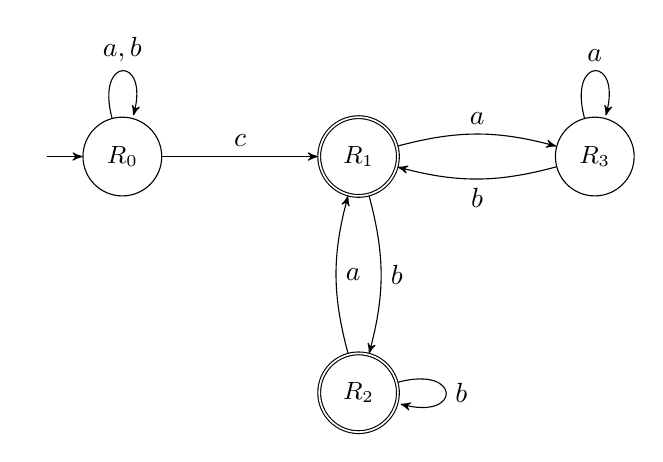
\begin{tikzpicture}[->, node distance=3.0cm, auto]
    \node[state, initial]    (R0) {$R_0$};
    \node[state, accepting]  (R1) [right of=R0] {$R_1$};
    \node[state, accepting]  (R2) [below of=R1] {$R_2$};
    \node[state]             (R3) [right of=R1] {$R_3$};
    \path
      (R0) edge [loop above] node {$a,b$} ()
      (R0) edge node {$c$} (R1)
      (R1) edge [bend left=15] node [above] {$a$} (R3)
      (R1) edge [bend left=15] node [right] {$b$} (R2)
      (R2) edge [bend left=15] node [right] {$a$} (R1)
      (R2) edge [loop right]   node {$b$} ()
      (R3) edge [loop above]   node {$a$} ()
      (R3) edge [bend left=15] node [below] {$b$} (R1);
  \end{tikzpicture}
  \caption{DFA mínimo para \rx{(a|b)*c(a+b|ba?)*}.
    $R_0{=}\{q_0\}$;
    $R_1{=}\{q_9,q_{10},q_{11},q_{12},q_{14},q_{22}\}^*$;
    $R_2{=}\{q_{11},q_{12},q_{13},q_{14},q_{22},q_{23},\ldots,q_{29}\}^*$;
    $R_3{=}\{q_{17},q_{18},q_{19},q_{20}\}$.}
  \label{fig:dfa-regex5}
\end{figure}

% =================================================================
\chapter{Parte 3 --- Atividade Complementar: Regex Crossword}
% =================================================================

\section{Introdução}

\textit{Regex Crossword} é uma plataforma de quebra-cabeças interativos
disponível em \url{https://regexcrossword.com}, na qual o objetivo é
preencher uma grade bidimensional com caracteres de modo que cada linha
e cada coluna satisfaça simultaneamente a expressão regular especificada
como restrição. A atividade exercita, de maneira lúdica, a capacidade
do aluno de construir e interpretar expressões regulares --- habilidade
central na disciplina de Teoria da Computação.

Este capítulo apresenta as soluções para os cinco desafios da seção
\textit{Beginner} e, em seguida, descreve dois quebra-cabeças originais
criados e publicados pelo aluno na seção \textit{Player Puzzles}.

% -----------------------------------------------------------------
\section{Desafios da Seção \textit{Beginner}}
% -----------------------------------------------------------------

A seção \textit{Beginner} compreende cinco desafios introdutórios, cada
um com grade 2×2. A Figura~\ref{fig:desafios-concluidos} apresenta a
visão geral dos cinco desafios concluídos.

\begin{figure}[H]
  \centering
  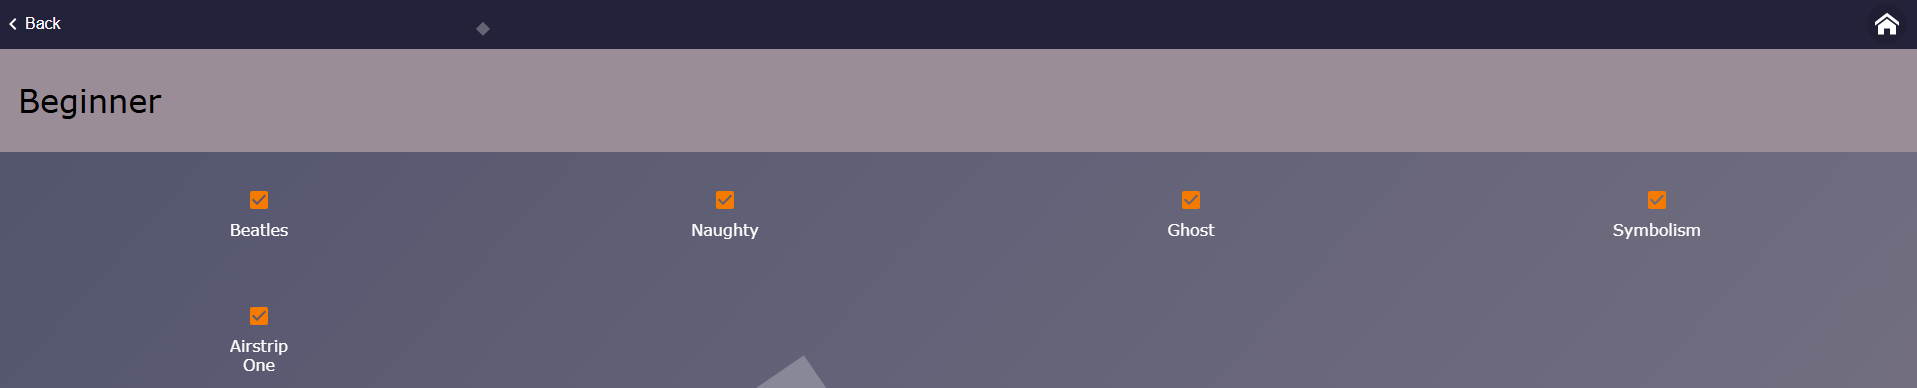
\includegraphics[width=0.9\textwidth]{img/regexcrossword_Desafios_Concluidos.png}
  \caption{Visão geral dos cinco desafios da seção \textit{Beginner}
    concluídos: Beatles, Naughty, Ghost, Symbolism e Airstrip One.}
  \label{fig:desafios-concluidos}
\end{figure}

% . . . . . . . . . . . . . . . . . . . . . . . . . . . . . . . .
\subsection{Desafio 1 --- \textit{Beatles}}

O desafio \textit{Beatles} apresenta restrições baseadas em alternância
e classes de caracteres. A solução é formada pelas letras
\celula{H}, \celula{E}, \celula{L}, \celula{P} --- compondo a palavra
\textit{HELP}, título do álbum homônimo dos Beatles de 1965.

\begin{figure}[H]
  \centering
  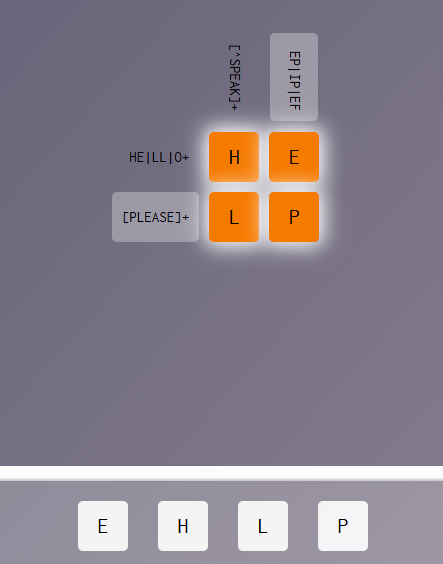
\includegraphics[width=0.38\textwidth]{img/Desafio_1.png}
  \caption{Desafio \textit{Beatles} --- solução: HELP.}
  \label{fig:desafio1}
\end{figure}

\begin{center}
\renewcommand{\arraystretch}{1.4}
\begin{tabular}{r|c|c|}
  \multicolumn{1}{r}{} &
  \multicolumn{1}{c}{\rx{HE|LL|O+}} &
  \multicolumn{1}{c}{\rx{[PLEASE]+}} \\
  \cline{2-3}
  \rx{[*SPEAK]+} & \celula{H} & \celula{E} \\
  \cline{2-3}
  \rx{EP|IP|EF}  & \celula{L} & \celula{P} \\
  \cline{2-3}
\end{tabular}
\end{center}

% . . . . . . . . . . . . . . . . . . . . . . . . . . . . . . . .
\subsection{Desafio 2 --- \textit{Naughty}}

O desafio \textit{Naughty} introduz o operador de referência reversa
(\rx{\textbackslash{}1}), que exige que determinada subcadeia coincida
com o grupo de captura anterior. A solução é
\celula{B}, \celula{O}, \celula{B}, \celula{E}.

\begin{figure}[H]
  \centering
  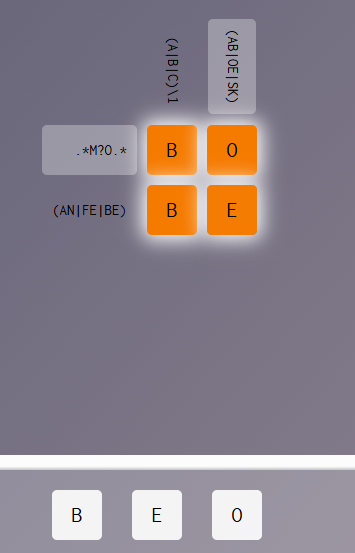
\includegraphics[width=0.38\textwidth]{img/Desafio_2.png}
  \caption{Desafio \textit{Naughty} --- solução: BOBE.}
  \label{fig:desafio2}
\end{figure}

\begin{center}
\renewcommand{\arraystretch}{1.4}
\begin{tabular}{r|c|c|}
  \multicolumn{1}{r}{} &
  \multicolumn{1}{c}{\rx{(A|B|C)\textbackslash{}1}} &
  \multicolumn{1}{c}{\rx{(AB|OE|SK)}} \\
  \cline{2-3}
  \rx{.*M?O.*}    & \celula{B} & \celula{O} \\
  \cline{2-3}
  \rx{(AN|FE|BE)} & \celula{B} & \celula{E} \\
  \cline{2-3}
\end{tabular}
\end{center}

Verificação das restrições:
\begin{itemize}
  \item Linha 1 (\textit{BO}): \rx{.*M?O.*} --- \texttt{B} casa \rx{.*},
    \rx{M?} é omitido (zero ocorrências), \texttt{O} casa literalmente \checkmark
  \item Linha 2 (\textit{BE}): \rx{(AN|FE|BE)} --- terceira alternativa \checkmark
  \item Coluna 1 (\textit{BB}): \rx{(A|B|C)\textbackslash{}1} --- grupo captura
    \texttt{B}, referência reversa exige novo \texttt{B} \checkmark
  \item Coluna 2 (\textit{OE}): \rx{(AB|OE|SK)} --- segunda alternativa \checkmark
\end{itemize}

% . . . . . . . . . . . . . . . . . . . . . . . . . . . . . . . .
\subsection{Desafio 3 --- \textit{Ghost}}

No desafio \textit{Ghost}, todas as quatro células recebem o caractere
\celula{O}, compondo a solução \textit{OOOO}.

\begin{figure}[H]
  \centering
  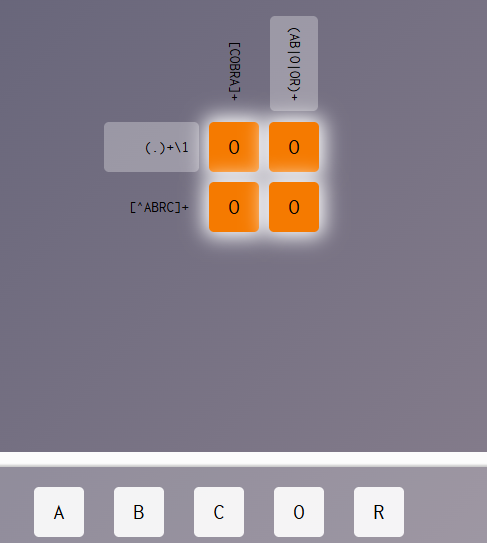
\includegraphics[width=0.38\textwidth]{img/Desafio_3.png}
  \caption{Desafio \textit{Ghost} --- solução: OOOO.}
  \label{fig:desafio3}
\end{figure}

\begin{center}
\renewcommand{\arraystretch}{1.4}
\begin{tabular}{r|c|c|}
  \multicolumn{1}{r}{} &
  \multicolumn{1}{c}{\rx{[COBRA]+}} &
  \multicolumn{1}{c}{\rx{(AB|O|OR)+}} \\
  \cline{2-3}
  \rx{(.)+\textbackslash{}1}       & \celula{O} & \celula{O} \\
  \cline{2-3}
  \rx{[\textasciicircum{}ABRC]+}   & \celula{O} & \celula{O} \\
  \cline{2-3}
\end{tabular}
\end{center}

Verificação:
\begin{itemize}
  \item Linha 1 (\textit{OO}): \rx{(.)+\textbackslash{}1} --- \rx{(.)} captura
    \texttt{O}, quantificador \rx{+} permite iteração, referência reversa
    exige novo \texttt{O} \checkmark
  \item Linha 2 (\textit{OO}): \rx{[\textasciicircum{}ABRC]+} ---
    \texttt{O} $\notin$ \{A, B, R, C\} \checkmark
  \item Coluna 1 (\textit{OO}): \rx{[COBRA]+} ---
    \texttt{O} $\in$ \{C, O, B, R, A\} \checkmark
  \item Coluna 2 (\textit{OO}): \rx{(AB|O|OR)+} --- alternativa \rx{O}
    aplicada duas vezes \checkmark
\end{itemize}

% . . . . . . . . . . . . . . . . . . . . . . . . . . . . . . . .
\subsection{Desafio 4 --- \textit{Symbolism}}

O desafio \textit{Symbolism} utiliza exclusivamente caracteres simbólicos
do alfabeto \{\rx{*}, \rx{+}, \rx{,}, \rx{/}\}. A solução é
\celula{*}, \celula{*}, \celula{/}, \celula{/}.

\begin{figure}[H]
  \centering
  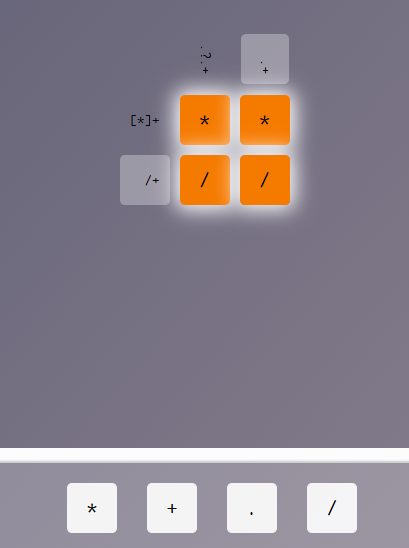
\includegraphics[width=0.38\textwidth]{img/Desafio_4.png}
  \caption{Desafio \textit{Symbolism} --- solução: \texttt{**/{}/ }.}
  \label{fig:desafio4}
\end{figure}

\begin{center}
\renewcommand{\arraystretch}{1.4}
\begin{tabular}{|c|c|}
  \hline
  \celula{*} & \celula{*} \\
  \hline
  \celula{/} & \celula{/} \\
  \hline
\end{tabular}
\end{center}

O desafio explora o fato de que, dentro de classes de caracteres
(\rx{[\ldots{}]}), quantificadores como \rx{*} e \rx{+} perdem seu
significado especial e são interpretados como literais. A restrição de
linha 2, \rx{/+}, exige um ou mais \rx{/} --- a sequência \textit{//}
satisfaz a expressão \checkmark.

% . . . . . . . . . . . . . . . . . . . . . . . . . . . . . . . .
\subsection{Desafio 5 --- \textit{Airstrip One}}

O desafio \textit{Airstrip One} utiliza dígitos do alfabeto
\{0, 1, 4, 6, 8, 9\}. A solução é
\celula{1}, \celula{9}, \celula{8}, \celula{4} --- compondo o número
\textit{1984}, referência ao romance distópico de George Orwell
(\textit{Airstrip One} é o nome dado à Inglaterra na obra).

\begin{figure}[H]
  \centering
  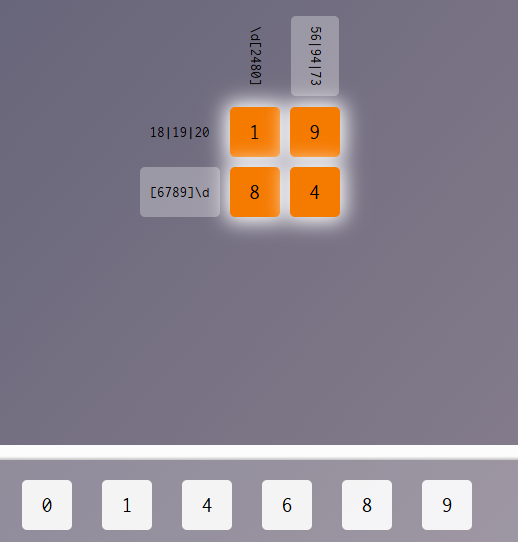
\includegraphics[width=0.38\textwidth]{img/Desafio_5.png}
  \caption{Desafio \textit{Airstrip One} --- solução: 1984.}
  \label{fig:desafio5}
\end{figure}

\begin{center}
\renewcommand{\arraystretch}{1.4}
\begin{tabular}{r|c|c|}
  \multicolumn{1}{r}{} &
  \multicolumn{1}{c}{\rx{\textbackslash{}d[2480]}} &
  \multicolumn{1}{c}{\rx{56|94|73}} \\
  \cline{2-3}
  \rx{18|19|20}               & \celula{1} & \celula{9} \\
  \cline{2-3}
  \rx{[6789]\textbackslash{}d} & \celula{8} & \celula{4} \\
  \cline{2-3}
\end{tabular}
\end{center}

Verificação:
\begin{itemize}
  \item Linha 1 (\textit{19}): \rx{18|19|20} --- segunda alternativa \checkmark
  \item Linha 2 (\textit{84}): \rx{[6789]\textbackslash{}d} ---
    \texttt{8} $\in$ \{6,7,8,9\}, \texttt{4} $\in \Sigma_{\text{dígitos}}$ \checkmark
  \item Coluna 1 (\textit{18}): \rx{\textbackslash{}d[2480]} ---
    \texttt{1} $\in \Sigma_{\text{dígitos}}$,
    \texttt{8} $\in$ \{2,4,8,0\} \checkmark
  \item Coluna 2 (\textit{94}): \rx{56|94|73} --- segunda alternativa \checkmark
\end{itemize}

% -----------------------------------------------------------------
\section{Quebra-cabeças Criados pelo Aluno}
% -----------------------------------------------------------------

Dois quebra-cabeças originais foram criados e publicados na seção
\textit{Player Puzzles} do \textit{Regex Crossword}. Ambos empregam
referências ao nome do autor e à instituição de ensino.

% . . . . . . . . . . . . . . . . . . . . . . . . . . . . . . . .
\subsection{Quebra-cabeça 1 --- FLAVIO\_HOUSE\_IFES (Grade 5×6)}

O quebra-cabeça \texttt{FLAVIO\_HOUSE\_IFES} é uma grade retangular de
5 linhas por 6 colunas, disponível em:
\begin{center}
  \url{https://regexcrossword.com/playerpuzzles/69ec93119f2fd}
\end{center}

As expressões regulares de linha foram projetadas para evocar palavras
associadas ao nome do autor, à família e ao lar. O alfabeto utilizado
inclui letras maiúsculas e o símbolo \heart{} como caractere especial.

\begin{figure}[H]
  \centering
  \noindent
  \begin{minipage}[b]{0.47\textwidth}
    \centering
    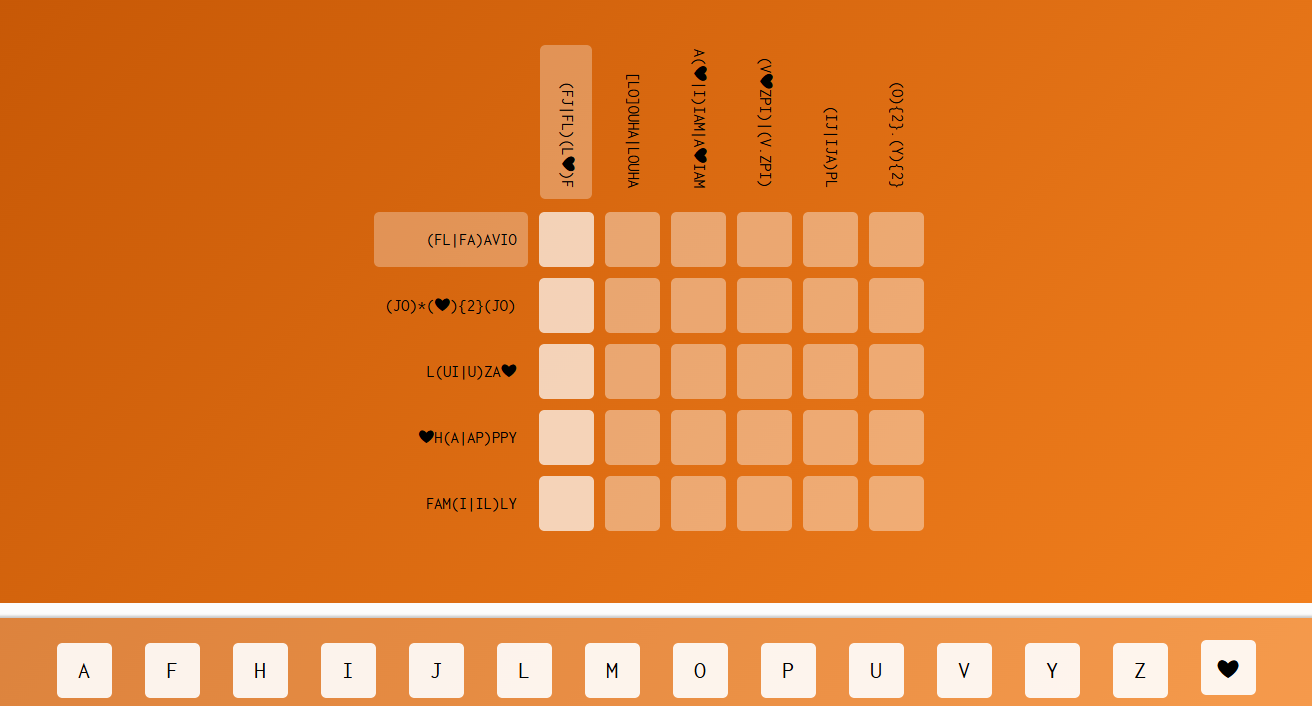
\includegraphics[width=\textwidth]{img/Player_Puzzles_FLAVIO_HOUSE_IFES_5X6.png}
    \small Quebra-cabeça sem solução.
  \end{minipage}
  \hfill
  \begin{minipage}[b]{0.47\textwidth}
    \centering
    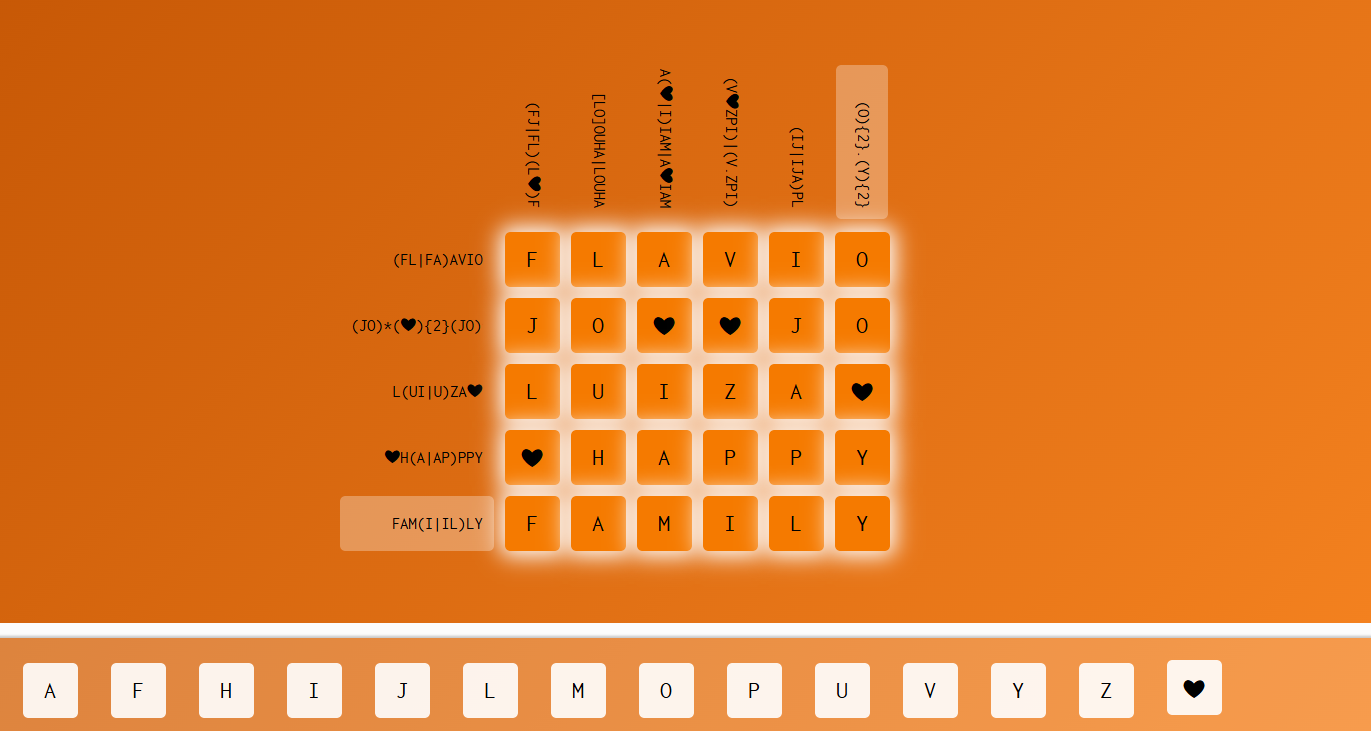
\includegraphics[width=\textwidth]{img/Player_Puzzles_FLAVIO_HOUSE_IFES_5X6_SOLVED.png}
    \small Quebra-cabeça com solução preenchida.
  \end{minipage}
  \caption{Quebra-cabeça FLAVIO\_HOUSE\_IFES --- grade retangular 5×6.}
  \label{fig:puzzle1}
\end{figure}

As restrições de linha projetadas são apresentadas na
Tabela~\ref{tab:puzzle1-linhas}.

\begin{table}[H]
  \centering
  \caption{Restrições de linha do quebra-cabeça FLAVIO\_HOUSE\_IFES.}
  \label{tab:puzzle1-linhas}
  \begin{tabular}{clp{5cm}}
    \toprule
    \textbf{Linha} & \textbf{Expressão Regular}        & \textbf{Solução} \\
    \midrule
    1 & \rx{(FL|FA)AVIO}                              & FLAVIO \\
    2 & \rx{(JO)+}\heart\rx{(2)(JO)}                  & JO\heart{}JO \\
    3 & \rx{L(UI|U)ZA}\heart                           & LUZA\heart \\
    4 & \heart\rx{H(A|AP)PPY}                          & \heart{}HAPPY \\
    5 & \rx{FAM(I|IL)Y}                               & FAMILY \\
    \bottomrule
  \end{tabular}
\end{table}

% . . . . . . . . . . . . . . . . . . . . . . . . . . . . . . . .
\subsection{Quebra-cabeça 2 --- FLAVIO\_MB\_IFES (Grade Hexagonal)}

O quebra-cabeça \texttt{FLAVIO\_MB\_IFES} é uma grade hexagonal de
tamanho 10 (arranjo 3-4-3), disponível em:
\begin{center}
  \url{https://regexcrossword.com/playerpuzzles/69ec8bdfb48b0}
\end{center}

A grade hexagonal impõe restrições em três direções --- linhas horizontais
e duas diagonais --- o que aumenta significativamente a complexidade do
design em relação a grades retangulares. O alfabeto utilizado é
\{C, E, F, I, J, M, O, P, S\}.

\begin{figure}[H]
  \centering
  \noindent
  \begin{minipage}[b]{0.47\textwidth}
    \centering
    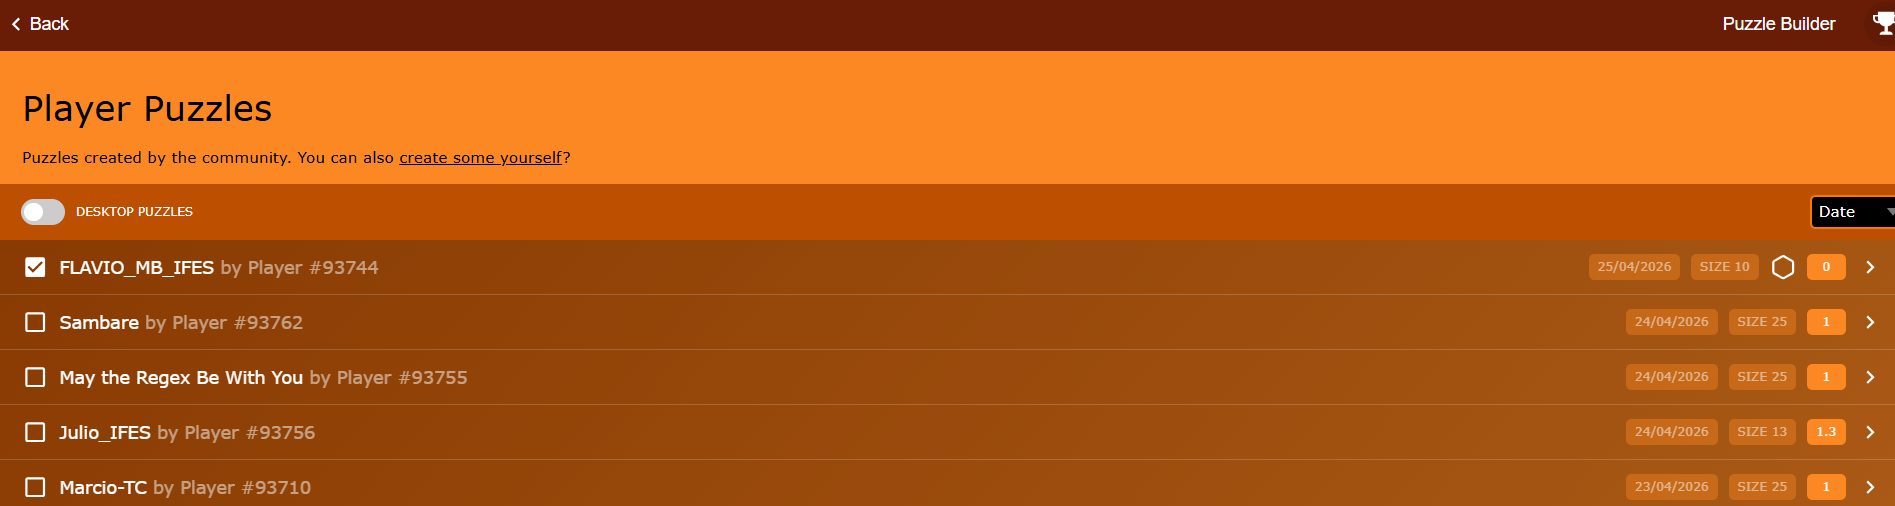
\includegraphics[width=\textwidth]{img/Player_Puzzles_FLAVIO_MB_IFES.png}
    \small Listagem do quebra-cabeça.
  \end{minipage}
  \hfill
  \begin{minipage}[b]{0.47\textwidth}
    \centering
    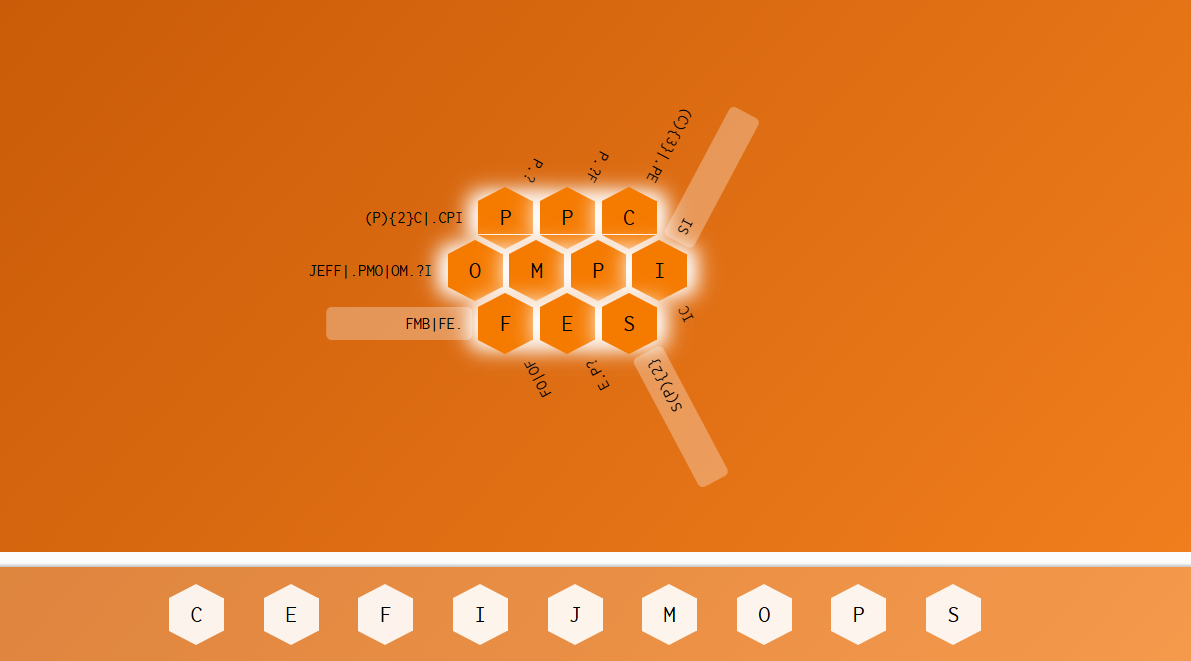
\includegraphics[width=\textwidth]{img/Player_Puzzles_FLAVIO_MB_IFES_Solved.png}
    \small Quebra-cabeça com solução preenchida.
  \end{minipage}
  \caption{Quebra-cabeça FLAVIO\_MB\_IFES --- grade hexagonal, tamanho 10.}
  \label{fig:puzzle2}
\end{figure}

A solução da grade hexagonal, lida linha a linha em arranjo 3-4-3, compõe:

\begin{center}
\renewcommand{\arraystretch}{1.3}
\begin{tabular}{ccc}
  Linha 1: & \celula{P} \celula{P} \celula{C}         & (3 células) \\
  Linha 2: & \celula{O} \celula{M} \celula{P} \celula{I} & (4 células) \\
  Linha 3: & \celula{F} \celula{E} \celula{S}         & (3 células) \\
\end{tabular}
\end{center}

O resultado --- \textit{PPCOMPIFES} --- é uma referência ao Programa de
Pós-Graduação em Computação Aplicada (PPCOMPI) do Instituto Federal do
Espírito Santo (IFES), programa ao qual o autor está vinculado. As
restrições de linha horizontais são apresentadas na
Tabela~\ref{tab:puzzle2-linhas}.

\begin{table}[H]
  \centering
  \caption{Restrições de linha do quebra-cabeça FLAVIO\_MB\_IFES.}
  \label{tab:puzzle2-linhas}
  \begin{tabular}{clp{5cm}}
    \toprule
    \textbf{Linha} & \textbf{Expressão Regular} & \textbf{Solução} \\
    \midrule
    1 & \rx{(P)(2)C|CPI}   & PPC \\
    2 & \rx{JEFF|PMO|OM?I}  & OMPI \\
    3 & \rx{FMB|FE.}        & FES \\
    \bottomrule
  \end{tabular}
\end{table}

\end{document}
